\chapter{Lecture 4 - Rankine Cycle Exergy Accounting}
\label{ch:ch4}
\section{Objectives}
The objectives of this lecture are:
\begin{itemize}
\item Illustrate exergy accounting with a simple Rankine cycle
\item Show how to carry out the calculations in a MATLAB environment using EasyProp.
\end{itemize}

\section{Simple Ideal Rankine Cycle - Exergy Accounting}
\newthought{Consider again} the Rankine cycle with system parameters specified to resemble a highly simplified version of a Westinghouse AP1000. A schematic of this system is given in Figure \ref{fig:simple_rankine_3}.
\begin{figure}
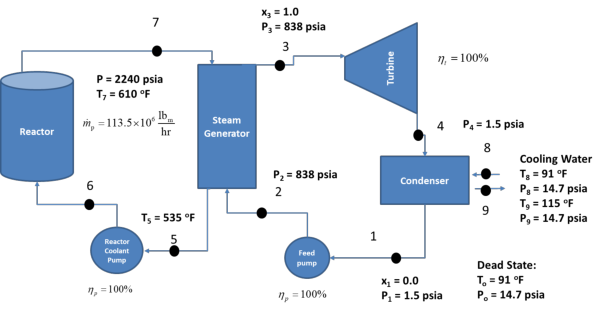
\includegraphics{simple_ideal_rankine.pdf}
\caption{Simple ideal Rankine cycle modeled on the Westinghouse AP1000.}
\label{fig:simple_rankine_3}
\end{figure}
Our goal is to carry out the exergy accounting as described in Lecture 3 for this system.  

\newthought{We will follow} a step-by-step process to complete this analysis.

\begin{enumerate}
\item Carry out the basic ``First Law'' of thermodynamics analysis for this system.  This was mostly done in Lecture 2;\sidenote{In Lecture 2 we did not include state points 5-9.  Data needed to find specific enthalpy and entropy for those state points are provided in Lecture 1.}  the details will not be repeated here except to remind you that we have instantiated an object to calculate thermodynamic properties of the working fluid, water:

\begin{lstlisting}[caption=Construct a \emph{simpleFluid} object]
units = 'USCS';
fluid = 'Water';
water = py.EasyProp.simpleFluid(fluid, units);
\end{lstlisting}

\item Determine dead state enthalpy ($h_o$) and entropy ($s_o$).  With the given dead state temperature and pressure, we can find this as follows:
\begin{lstlisting}[caption=Find dead state enthalpy and entropy]
To_F = 91; % F, dead state temp
Po = 14.7; % psia, dead state pressure
ho = water.h_pT(Po,To_F);
so = water.s_pT(Po,To_F);
To = To_F + 460; % R, dead state absolute temperature
\end{lstlisting}
Note that EasyProp functions require the temperature in either C or F, but the $T_o$ appearing in the specific flow exergy equations must be in absolute units: K or R.
%\begin{marginfigure}
%
\includegraphics{bug-icon.png}
%\end{marginfigure}

\item Calculate the specific flow exergy for all state points.  You should calculate all state point enthalpy and entropy values as part of your ``First Law'' analysis.  In MATLAB one can then create an in-line function to quickly calculate the specific flow exergy for all state points.

\begin{lstlisting}[caption=Compute specific flow exergy for all state points]
ef_fun = @(h,s) (h - ho) - To*(s - so);
ef = ef_fun(h,s); % BTU/lbm, specific flow exergy 
\end{lstlisting}
Note that the arrays for $h$ and $s$ should be populated with the correct enthalpy and entropy for all state points before this calculation is made.
\item Calculate the exergy destruction rate for each process.  In each process this is calculated from a re-arrangement of the exergy balance equation given in Lecture 3:

\begin{equation}
\dot{E}_d = \sum_{i}\dot{m}_i e_{f_i} - \sum_{e} \dot{m}_e e_{f_e} - \dot{W}
\label{eq:ex_d_eqn}
\end{equation}

In this cycle there are four processes to consider:
\begin{enumerate}
\item \textbf{Exergy destruction rate in the steam generator.}  Focus on the relevant process showing in Figure \ref{fig:SIR_sg}.  The steam generator has two in-flows and two exits; one each from the primary and secondary side.  For this particular problem we are only given the mass flow rate of the primary ($\dot{m}_p$) so we first need to get the mass flow rate in the secondary.  This can be obtained from simple conservation of energy principles:
$$ \dot{m}_s(h_3 - h_2) = \dot{m}_p(h_7 - h_5)$$

\begin{marginfigure}
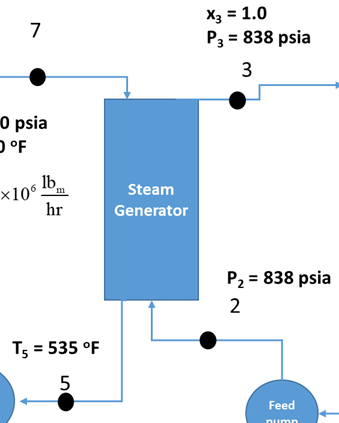
\includegraphics{SIR_sg.png}
\caption{Constant pressure heat transfer process in the steam generator}
\label{fig:SIR_sg}
\end{marginfigure}
\begin{lstlisting}
m_s = m_p*(h_7 - h_6)/(h_3 - h_2); % lbm/hr, mass flow rate through S/G.
\end{lstlisting}
Now, using Equation \ref{eq:ex_d_eqn}, we compute the exergy destruction rate:

\begin{lstlisting}
Ex_d_sg = m_p*ef(7) + m_s*ef(2) - (m_p*ef(5) + m_s*ef(3)); % BTU/hr
\end{lstlisting}
Note that since there is no work done in the steam generator, there is no exergy transfer through work.

\item \textbf{Exergy destruction rate in the turbine.} The relevant process here is shown in Figure \ref{fig:SIR_turb}.  Note that since there is work being done in the turbine, there is exergy transfer through work that we need to take into account.
\begin{marginfigure}
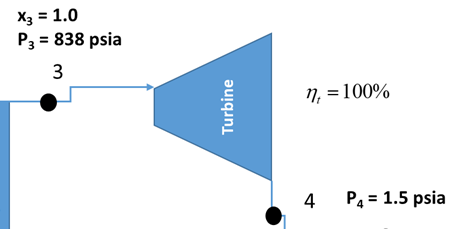
\includegraphics{SIR_turb.png}
\caption{Expansion of the working fluid in the turbine.}
\label{fig:SIR_turb}
\end{marginfigure}
\begin{lstlisting}
Ex_d_turb = m_s*(ef(3) - ef(4)) - m_s*w_turb; % BTU/hr 
\end{lstlisting}
Here we expect $w_{turb}$, the specific work of the turbine, to have previously been calculated in the ``First Law'' analysis as $w_{turb} = h(3) - h(4)$.\sidenote[][-1.25cm]{\textbf{Note: }for this simple ideal cycle, you should find that the exergy destruction rate for the ideal turbine to be zero!}

\item \textbf{Exergy destruction rate in the condenser.}  Analysis of the condenser is much like the steam generator: two in-flows and two exit-flows and no work done in the process.  Also in this case, like the steam generator, we need to use conservation of energy to determine the required flow rate of the condenser cooling water $\dot{m}_c$.  The relevant process schematic is illustrated in Figure \ref{fig:SIR_cond}.

\begin{marginfigure}
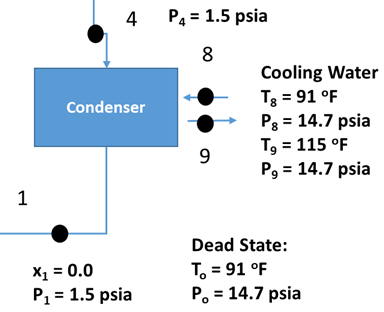
\includegraphics{SIR_cond.png}
\caption{Constant pressure heat rejection in the condenser.}
\label{fig:SIR_cond}
\end{marginfigure}

\begin{lstlisting}
m_c = m_s*(h(4) - h(1))/(h(9)-h(8)); % lbm/hr, condenser cooling water flow

Ex_d_cnd = m_c*ef(8) + m_s*ef(4) - (m_c*ef(9) + m_s*ef(1)); % BTU/hr
\end{lstlisting}

\item Exergy destruction rate in the feed pump.  Like the turbine, the feed pump has one inlet and one exit and there is also exergy transfer through work. The relevant process schematic is illustrated in Figure \ref{fig:SIR_mfp}. The MATLAB code would be:
\begin{marginfigure}
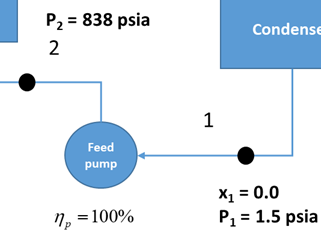
\includegraphics{SIR_mfp.png}
\caption{Work in to the working fluid from the feed pump.}
\label{fig:SIR_mfp}
\end{marginfigure}
\begin{lstlisting}
Ex_d_fp = m_s*(ef(1) - ef(2)) - m_s*w_fp; % BTU/hr
\end{lstlisting}
where $w_{fp}$ would be calculated simply as $w_{fp} = h(1) - h(2)$.  

\end{enumerate}

\item Calculate the ``Exergy In'' to the system from the primary coolant and ``Exergy Out'' from the system to the environment via the condenser.  For the Exergy In we will simply use the mass flow rate of primary coolant times the change in specific flow exergy of the primary coolant through the steam generator; for Exergy Out we will use the mass flow rate of condenser cooling water times the increase in specific flow exergy of the water.

\begin{lstlisting}
Ex_in = m_p*(ef(7) - ef(6)); % BTU/lbm
Ex_out = m_c*(ef(9) - ef(8)); % BTU/lbm
\end{lstlisting}

\item Verify the overall exergy balance.  The balance should look something like:

\begin{lstlisting}
balance = Ex_in - Ex_out - m_s*w_net - ...
          (Ex_d_sg + Ex_d_cnd + Ex_d_turb + Ex_d_fp);
\end{lstlisting}

\end{enumerate}

If everything is correct and if you have not violated the Second Law of Thermodynamics the computed balance should be zero.  In exactly the same way that you should verify that net specific work is the same as net specific heat transferred ($w_{net} = q_{net}$) --- thereby satisfying conservation of energy (First Law of Thermodynamics) --- you should check the balance on the exergy analysis to ensure you have satisfied the Second Law of Thermodynamics.

